\chapter{Introduction}

\section{Cryptography and Side Channel Attacks}
Cryptography derived from solving the problem of transmitting secret information through an insecure channel. The general principle  in modern cryptography is that the encryption and decryption algorithms are assumed to be made public and the secrecy of messages is solely relied on the secrecy of the key. 

Under this assumption, cryptographic algorithms are then designed in various ways. Some of them are derived from hard mathematical problems such as Discrete Logarithm and Elliptic Curves. Provable Security provides mathematical proofs by modelling the algorithms in an abstracted mathematical world and reduces them to hard problems; the secrecy of message is then guaranteed as long as the underlying mathematical problems are not solved.

However, when implemented in real world things can get out of control. Many factors considered difficult to be modelled mathematically can sometimes be exploited to breach the security. For example, \cite{DPA} describes a method called Differential Power Analysis which recovers the secret key using power traces measured during encryption; \cite{Cache-Timing1} and \cite{Cache-Timing2} shows that the timing information can also  reveal the secret key.

\section{Network Traffic}
The conceptional structure of today’s network is described in \cite{OSI}. Generally speaking, networks are formed by protocols which are standard agreements implemented by nodes connected to the networks. Protocols are categorised as a stack of layer with the lower ones handle the fussy transportation  problems and the higher ones the more sophisticated functional problems. 

Packet (or frame) is the unit of structured data transmitted through network at each layer. A typical format of packet is a protocol header followed by its payload. The header constitutes of several fields which contain some meta data of the packet while the payload is the actual data being transmitted. 

\begin{table}[H]
\begin{center}
{\begin{tabular}{l|l|l|}
\cline{2-3}
                  & Layer             & Example Protocols        \\ \cline{2-3} 
High            & Application Layer & HTTP / SMTP / NTP        \\ \cline{2-3} 
  & Secure Layer      & TLS / SSL / DTLS         \\ \cline{2-3} 
              & Transport Layer   & TCP / UDP / SCTP         \\ \cline{2-3} 
              & Network Layer     & IPv4 / IPv6 / 6lowPAN    \\ \cline{2-3} 
               & Data Link Layer   & IEEE 802.3 / IEEE 802.11 \\ \cline{2-3} 
Low                 & Physical Layer    &  Bluetooth / DSL        \\ \cline{2-3} 
\end{tabular}
}
\end{center}
\caption{A Simplified 6 Layer Model}
\label{Tbl: OSI}
\end{table}

Packet of protocols are organised recursively, i.e. headers of upper protocols is embedded into the payload of lower protocols. When a packet (or frame) arrives a node on the network, the headers are decapsulated sequentially from the lowest layer to the highest. Conceptional speaking, the content of a payload should be transparent to the protocols beneath. For instance, a router may only decapsulate a packet no higher than IP layer and has no concern about everything above.

\begin{figure}[H]
\centering
\resizebox{12cm}{!}
{% Graphic for TeX using PGF
% Title: /home/yy12135/Writings/First-year-review_20150422/Pics/HeaderPayload.dia
% Creator: Dia v0.97.2
% CreationDate: Wed Apr  1 16:51:21 2015
% For: yy12135
% \usepackage{tikz}
% The following commands are not supported in PSTricks at present
% We define them conditionally, so when they are implemented,
% this pgf file will use them.
\ifx\du\undefined
  \newlength{\du}
\fi
\setlength{\du}{15\unitlength}
\begin{tikzpicture}
\pgftransformxscale{1.000000}
\pgftransformyscale{-1.000000}
\definecolor{dialinecolor}{rgb}{0.000000, 0.000000, 0.000000}
\pgfsetstrokecolor{dialinecolor}
\definecolor{dialinecolor}{rgb}{1.000000, 1.000000, 1.000000}
\pgfsetfillcolor{dialinecolor}
\definecolor{dialinecolor}{rgb}{1.000000, 1.000000, 1.000000}
\pgfsetfillcolor{dialinecolor}
\fill (15.787500\du,22.000000\du)--(15.787500\du,23.900000\du)--(20.000000\du,23.900000\du)--(20.000000\du,22.000000\du)--cycle;
\pgfsetlinewidth{0.100000\du}
\pgfsetdash{}{0pt}
\pgfsetdash{}{0pt}
\pgfsetmiterjoin
\definecolor{dialinecolor}{rgb}{0.000000, 0.000000, 0.000000}
\pgfsetstrokecolor{dialinecolor}
\draw (15.787500\du,22.000000\du)--(15.787500\du,23.900000\du)--(20.000000\du,23.900000\du)--(20.000000\du,22.000000\du)--cycle;
% setfont left to latex
\definecolor{dialinecolor}{rgb}{0.000000, 0.000000, 0.000000}
\pgfsetstrokecolor{dialinecolor}
\node at (17.893750\du,23.145000\du){IP Header};
\definecolor{dialinecolor}{rgb}{1.000000, 1.000000, 1.000000}
\pgfsetfillcolor{dialinecolor}
\fill (20.000000\du,22.000000\du)--(20.000000\du,23.900000\du)--(25.000000\du,23.900000\du)--(25.000000\du,22.000000\du)--cycle;
\pgfsetlinewidth{0.100000\du}
\pgfsetdash{}{0pt}
\pgfsetdash{}{0pt}
\pgfsetmiterjoin
\definecolor{dialinecolor}{rgb}{0.000000, 0.000000, 0.000000}
\pgfsetstrokecolor{dialinecolor}
\draw (20.000000\du,22.000000\du)--(20.000000\du,23.900000\du)--(25.000000\du,23.900000\du)--(25.000000\du,22.000000\du)--cycle;
% setfont left to latex
\definecolor{dialinecolor}{rgb}{0.000000, 0.000000, 0.000000}
\pgfsetstrokecolor{dialinecolor}
\node at (22.500000\du,23.145000\du){TCP Header};
\definecolor{dialinecolor}{rgb}{1.000000, 1.000000, 1.000000}
\pgfsetfillcolor{dialinecolor}
\fill (25.000000\du,22.000000\du)--(25.000000\du,23.900000\du)--(31.000000\du,23.900000\du)--(31.000000\du,22.000000\du)--cycle;
\pgfsetlinewidth{0.100000\du}
\pgfsetdash{}{0pt}
\pgfsetdash{}{0pt}
\pgfsetmiterjoin
\definecolor{dialinecolor}{rgb}{0.000000, 0.000000, 0.000000}
\pgfsetstrokecolor{dialinecolor}
\draw (25.000000\du,22.000000\du)--(25.000000\du,23.900000\du)--(31.000000\du,23.900000\du)--(31.000000\du,22.000000\du)--cycle;
% setfont left to latex
\definecolor{dialinecolor}{rgb}{0.000000, 0.000000, 0.000000}
\pgfsetstrokecolor{dialinecolor}
\node at (28.000000\du,23.145000\du){TLS Header};
\definecolor{dialinecolor}{rgb}{1.000000, 1.000000, 1.000000}
\pgfsetfillcolor{dialinecolor}
\fill (31.000000\du,22.000000\du)--(31.000000\du,23.900000\du)--(40.000000\du,23.900000\du)--(40.000000\du,22.000000\du)--cycle;
\pgfsetlinewidth{0.100000\du}
\pgfsetdash{}{0pt}
\pgfsetdash{}{0pt}
\pgfsetmiterjoin
\definecolor{dialinecolor}{rgb}{0.000000, 0.000000, 0.000000}
\pgfsetstrokecolor{dialinecolor}
\draw (31.000000\du,22.000000\du)--(31.000000\du,23.900000\du)--(40.000000\du,23.900000\du)--(40.000000\du,22.000000\du)--cycle;
% setfont left to latex
\definecolor{dialinecolor}{rgb}{0.000000, 0.000000, 0.000000}
\pgfsetstrokecolor{dialinecolor}
\node at (35.500000\du,23.145000\du){......};
\pgfsetlinewidth{0.100000\du}
\pgfsetdash{}{0pt}
\pgfsetdash{}{0pt}
\pgfsetbuttcap
{
\definecolor{dialinecolor}{rgb}{0.000000, 0.000000, 0.000000}
\pgfsetfillcolor{dialinecolor}
% was here!!!
\pgfsetarrowsstart{to}
\pgfsetarrowsend{to}
\definecolor{dialinecolor}{rgb}{0.000000, 0.000000, 0.000000}
\pgfsetstrokecolor{dialinecolor}
\draw (31.000000\du,21.000000\du)--(40.000000\du,21.000000\du);
}
% setfont left to latex
\definecolor{dialinecolor}{rgb}{0.000000, 0.000000, 0.000000}
\pgfsetstrokecolor{dialinecolor}
\node[anchor=west] at (34.000000\du,20.000000\du){TLS payload};
\pgfsetlinewidth{0.100000\du}
\pgfsetdash{}{0pt}
\pgfsetdash{}{0pt}
\pgfsetbuttcap
{
\definecolor{dialinecolor}{rgb}{0.000000, 0.000000, 0.000000}
\pgfsetfillcolor{dialinecolor}
% was here!!!
\pgfsetarrowsstart{to}
\pgfsetarrowsend{to}
\definecolor{dialinecolor}{rgb}{0.000000, 0.000000, 0.000000}
\pgfsetstrokecolor{dialinecolor}
\draw (25.000000\du,19.000000\du)--(40.000000\du,19.000000\du);
}
% setfont left to latex
\definecolor{dialinecolor}{rgb}{0.000000, 0.000000, 0.000000}
\pgfsetstrokecolor{dialinecolor}
\node[anchor=west] at (31.000000\du,18.000000\du){TCP payload};
\pgfsetlinewidth{0.100000\du}
\pgfsetdash{}{0pt}
\pgfsetdash{}{0pt}
\pgfsetbuttcap
{
\definecolor{dialinecolor}{rgb}{0.000000, 0.000000, 0.000000}
\pgfsetfillcolor{dialinecolor}
% was here!!!
\pgfsetarrowsstart{to}
\pgfsetarrowsend{to}
\definecolor{dialinecolor}{rgb}{0.000000, 0.000000, 0.000000}
\pgfsetstrokecolor{dialinecolor}
\draw (20.000000\du,17.000000\du)--(40.000000\du,17.000000\du);
}
% setfont left to latex
\definecolor{dialinecolor}{rgb}{0.000000, 0.000000, 0.000000}
\pgfsetstrokecolor{dialinecolor}
\node[anchor=west] at (28.000000\du,16.000000\du){IP payload};
\pgfsetlinewidth{0.100000\du}
\pgfsetdash{{\pgflinewidth}{0.200000\du}}{0cm}
\pgfsetdash{{\pgflinewidth}{0.200000\du}}{0cm}
\pgfsetbuttcap
{
\definecolor{dialinecolor}{rgb}{0.000000, 0.000000, 0.000000}
\pgfsetfillcolor{dialinecolor}
% was here!!!
\definecolor{dialinecolor}{rgb}{0.000000, 0.000000, 0.000000}
\pgfsetstrokecolor{dialinecolor}
\draw (40.000000\du,16.000000\du)--(40.000000\du,25.000000\du);
}
\pgfsetlinewidth{0.100000\du}
\pgfsetdash{{\pgflinewidth}{0.200000\du}}{0cm}
\pgfsetdash{{\pgflinewidth}{0.200000\du}}{0cm}
\pgfsetbuttcap
{
\definecolor{dialinecolor}{rgb}{0.000000, 0.000000, 0.000000}
\pgfsetfillcolor{dialinecolor}
% was here!!!
\definecolor{dialinecolor}{rgb}{0.000000, 0.000000, 0.000000}
\pgfsetstrokecolor{dialinecolor}
\draw (31.000000\du,20.000000\du)--(31.000000\du,25.000000\du);
}
\pgfsetlinewidth{0.100000\du}
\pgfsetdash{{\pgflinewidth}{0.200000\du}}{0cm}
\pgfsetdash{{\pgflinewidth}{0.200000\du}}{0cm}
\pgfsetbuttcap
{
\definecolor{dialinecolor}{rgb}{0.000000, 0.000000, 0.000000}
\pgfsetfillcolor{dialinecolor}
% was here!!!
\definecolor{dialinecolor}{rgb}{0.000000, 0.000000, 0.000000}
\pgfsetstrokecolor{dialinecolor}
\draw (25.000000\du,18.000000\du)--(25.000000\du,25.000000\du);
}
\pgfsetlinewidth{0.100000\du}
\pgfsetdash{{\pgflinewidth}{0.200000\du}}{0cm}
\pgfsetdash{{\pgflinewidth}{0.200000\du}}{0cm}
\pgfsetbuttcap
{
\definecolor{dialinecolor}{rgb}{0.000000, 0.000000, 0.000000}
\pgfsetfillcolor{dialinecolor}
% was here!!!
\definecolor{dialinecolor}{rgb}{0.000000, 0.000000, 0.000000}
\pgfsetstrokecolor{dialinecolor}
\draw (20.000000\du,16.000000\du)--(20.000000\du,25.000000\du);
}
\end{tikzpicture}
}
\caption{An example of headers and payloads}
\label{Fig: Header and payloads}
\end{figure}

It might be difficult in real world to prevent a third party from seeing a packet. For example, a packet from your laptop cannot reach Google server without hopping between routers and hence any corrupted router may breach the data; the enriching application of mobile devices made it even more difficult as the radio signals from one’s smart phone can be captured easily in a cafe.

\section{Side Channel Information in Packets}
Theoretically speaking, encryption can be applied at any layer of a network. Lower the layer it is, more information is protected. However, the intense requirement of efficiency and bandwidth have limited the usage of cryptography, like IPSec. A trade-off between security and efficiency must be made and encryption at higher level protocol has eventuall adopted as a widely accepted solution. As a result, TLS/SSL has became the most used security protocol on Internet today.

The drawback, as mentioned above, is that all headers in the lower layers will be transmitted in plaintext. \Cref{Fig: Sniffer} is an example of a captured DTLS packet. 

\begin{figure}[H] 
\centering
\resizebox{12cm}{!}
{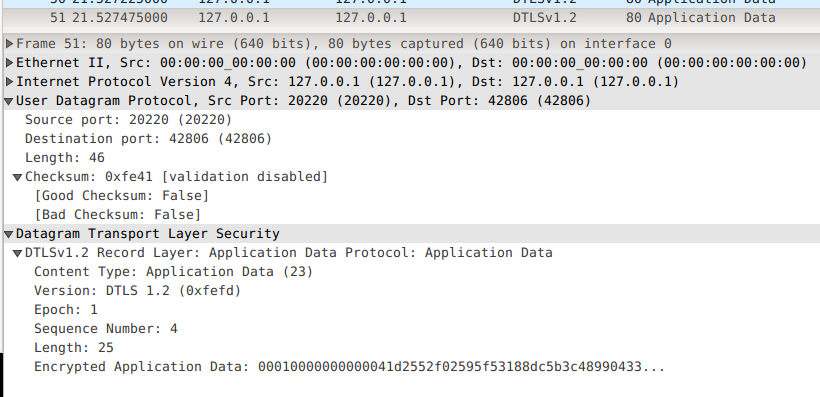
\includegraphics{./Pics/Sniffer.png}}
\caption{A Wireshark Screenshot}
\label{Fig: Sniffer}
\end{figure}

As we can see in  \Cref{Fig: Sniffer}, although the sniffer is not able to decrypt the packet, all headers until DTLS are indeed accessible.

\section{Motivation and Challenges}
The open nature of the development Internet of Things (IoT) demands more security and privacy measure. Unlike the stable and already-widely-deployed Internet, the structure of IoT network is still under a developing process; therefore it might be worthwhile to take into concern the security from an early stage.

One challenge in this project is the fundamental nature difference between network traffic and other physical side channel information. Many side channel attacks are aimed to recover secret key materials, such as DPA in \cite{DPA}, or Cache-timing Attack in \cite{Cache-Timing1} and \cite{Cache-Timing2}. 

Although it is not certain at this stage that whether there is a link between the value of cryptographic key chosen and packet headers, but intuitively they are more likely to be independent. The reason is that the cryptography primitives chosen should only affect the value of ciphertext which constitutes the payload; hence is expected to be transparent to the lower layer protocol headers. However, the timing information might still be exploited to recover the key material.

Different protocol suite result into different headers and hence different information. As a beginning for this project, we choose to study the traffic generated by a DTLS implementation called tinyDTLS\cite{tinyDTLS}. tinyDTLS is designed to be suitable for embedded systems and is one of the IoT candidates in the future.

%At current stage, we have developed a toy network application(\Cref{Chp: Toys}) to show that such potential of information leakage exists and demonstrated an attack method against the application. 

%The long term proposal of this project is to study what kind of information can be leaked through these unprotected meta data as well as any other kinds of  information an adversary can learn by simply capturing the network traffic. 